\documentclass[tikz,border=0pt]{standalone}
\usepackage{graphicx,amsmath}
\definecolor{navy}{HTML}{17365D}
\begin{document}
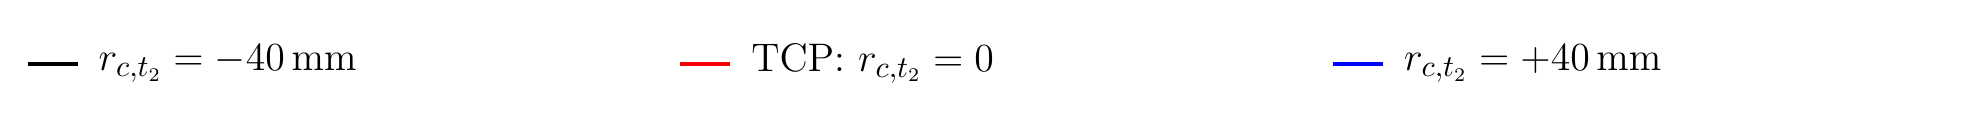
\begin{tikzpicture}[x=1bp,y=1bp]
\path[use as bounding box] (0,0) rectangle (690,26);
\draw[black,line width=1.3bp] (0,13)--(18,13);\node[anchor=west,font=\fontsize{15}{17}\selectfont] at (22,13) {$r_{c,t_2}=-40\,\mathrm{mm}$};
\draw[red,line width=1.3bp] (235,13)--(253,13);\node[anchor=west,font=\fontsize{15}{17}\selectfont] at (257,13) {TCP: $r_{c,t_2}=0$};
\draw[blue,line width=1.3bp] (470,13)--(488,13);\node[anchor=west,font=\fontsize{15}{17}\selectfont] at (492,13) {$r_{c,t_2}=+40\,\mathrm{mm}$};
\end{tikzpicture}
\end{document}
